% !TEX TS-program = pdflatex
% !TEX encoding = UTF-8 Unicode
% !TEX root = main.tex
% !TEX spellcheck = en-US
% ****************************************************************************************
% File: main.tex
% Author: Jakob Spindler
% Date: 2024-10-16
% ****************************************************************************************
\documentclass[a4paper,11pt,oneside,final,titlepage,openany,onecolumn]{report}
% input preamble (include additional packages, set options, define macros)
% !TEX TS-program = pdflatex
% !TEX encoding = UTF-8 Unicode
% !TEX root = ../main.tex
% !TEX spellcheck = en-US
% ****************************************************************************************
% File: _preamble.tex
% Author: Jakob Spindler
% Date: 2024-10-16
% ****************************************************************************************
% ****************************************************************************************
% General settings (input encoding, font encoding, font, language)
% ****************************************************************************************
\usepackage[utf8]{inputenc} % character encoding used in input file
\usepackage[T1]{fontenc} % specifies the encoding used in the fonts
\usepackage{lmodern} % provides more support for non-ASCII characters than cm-super
\usepackage{microtype} % improves line-filling when using PDFLaTeX
\usepackage[ngerman,english]{babel} %  last language is considered the main one
\renewcommand{\familydefault}{\sfdefault} % select a sans serif font family 

% \pdfsuppresswarningpagegroup=1 % suppress warning when including PDFs with page groups

% ****************************************************************************************
% Basic macros for thesis
% ****************************************************************************************
\newcommand{\authorName}{Jakob Spindler}
\newcommand{\authorContact}{sj0458@mci4me.at}

\newcommand{\department}{Department of Technology \& Life Sciences}
\newcommand{\docTitle}{Conducted Emissions of a Buck Converter}
\newcommand{\docType}{Report}
\newcommand{\studyProgram}{Master's program Mechatronics \& Smart Technologies}
\newcommand{\degree}{Master of Science in Engineering}
\newcommand{\studyYear}{MA-MECH-23-VZ}
\newcommand{\supervisorName}{Thomas Gadner}
\newcommand{\supervisorContact}{}
\newcommand{\assesorName}{Dr. Georg Saxl}
\newcommand{\assesorContact}{georg.saxl@mci.edu}
\newcommand{\university}{Management Center Innsbruck}
\newcommand{\matnr}{11941482}


\newcommand{\authorAName}{Liam Nolan}
\newcommand{\authorAContact}{nl6496@mci4me.at}
\newcommand{\authorBName}{Johannes Schmid}
\newcommand{\authorBContact}{sj0751@mci4me.at}
\newcommand{\authorCName}{Jakob Spindler}
%\newcommand{\authorCContact}{sj0458@mci4me.at}
\newcommand{\courseName}{WS 2024 Industrial Electronics}
\newcommand{\courseCode}{MECH-M-3-IEL-IEL-ILV}
%\newcommand{\department}{Department of Technology \& Life Sciences}
%\newcommand{\docTitle}{Optimization Study of a flow heater}
%\newcommand{\docType}{Report}
%\newcommand{\studyProgram}{Master's program Mechatronics \& Smart Technologies}
%\newcommand{\studyYear}{MA-MECH-23-VZ}
\newcommand{\lecturerName}{Manuel Berger, PhD}
\newcommand{\lecturerContact}{manuel.berger@mci.edu}
%\newcommand{\university}{Management Center Innsbruck}
% Definition of BibTeX macro used in IEEEexample
\newcommand{\BibTeX}{BibTeX}

% ****************************************************************************************
% Drawing and plotting, scientific packages, 
% ****************************************************************************************
% For use of subfigure environment
\usepackage{subcaption}

% For use of cmidrule in table environment
\usepackage{booktabs}

\usepackage{makecell}

% Handling of images
\usepackage{graphicx}
\graphicspath{{./img/}}

% Colour support
\usepackage[table]{xcolor}

% Handling of MATLAB code
%\usepackage{mcode}

% Tabulars with adjustable-width columns
\usepackage{tabularx}
\usepackage{multirow}

% Sketching and importing MATLAB plots
\usepackage{pgfplots}
\usepackage{grffile}
\pgfplotsset{compat=newest}
\usetikzlibrary{plotmarks}
\usetikzlibrary{arrows.meta}
\usetikzlibrary{patterns}
\usepgfplotslibrary{patchplots}
\pgfplotsset{plot coordinates/math parser=false}
\newlength\figureheight
\newlength\figurewidth

% Typesetting electrical networks
\usepackage{circuitikz}

% scientific packages
\usepackage{amsmath}
\usepackage{amsfonts}
\usepackage{xfrac}
\usepackage{siunitx}
\AtBeginDocument{\sisetup{
		mode=match,
		unit-font-command = \mathrm,
		reset-text-family=false,
		reset-text-series=false,
		reset-text-shape=false,
		exponent-product=\cdot
	}}
\DeclareSIUnit\unity{1} % can be used for dimensionless quantities
\DeclareSIUnit\sample{Sa}
% ****************************************************************************************
% Referencing and citing
% ****************************************************************************************
% Caption settings
\usepackage[
	format=plain, % typeset as normal paragraph
	labelformat=simple, % typeset label as name and number
	labelsep=period, % caption label and text separated by period and space
	textformat=simple, % caption text typeset as is
	justification=justified, % typset caption as normal paragraph
	singlelinecheck=true, % automatically center short captions
	font=small,
	labelfont=bf, % set bold font for label
	width=.75\textwidth % set fixed width for caption
]{caption}
\captionsetup[table]{position=top}
\captionsetup[figure]{position=bottom}

% Hypertext marks (should be loaded last but before geometry)
\usepackage[hyperindex]{hyperref}
% Extension options
\hypersetup{
	colorlinks, % colours the text of links and anchors (instead of borders)
	linkcolor={blue!65!black},
	citecolor={blue!65!black},
	urlcolor={blue!65!black}
}
% PDF display and information options
\hypersetup{
	pdftitle={\docTitle},
	pdfsubject={\docType},
	pdfauthor={\authorName},
	pdfkeywords={},
	pdfcreator={pdflatex},
	pdfproducer={LaTeX with hyperref}
}

% formatting of cross-references
\usepackage[capitalise]{cleveref}
\crefformat{equation}{(#2#1#3)}
\Crefformat{equation}{Equation~(#2#1#3)}

%matlab prettifier
\usepackage{matlab-prettifier}

% ****************************************************************************************
% Bibliography settings
% ****************************************************************************************
% template from https://www.ieee.org/conferences/publishing/templates.html
\usepackage[
	backend=biber,
	style=numeric-comp, % numeric style with compact multiple citations i.e. [1-5] and not [1,2,3,4,5]
	natbib=true,
	sorting=none
]{biblatex}
\addbibresource{bib.bib}


% ****************************************************************************************
% Glossary (acronyms, list of symbols) settings
% ****************************************************************************************
\usepackage[acronym,nomain,nonumberlist,nopostdot,sort=def,toc]{glossaries}
\renewcommand*{\glstextformat}[1]{\textcolor{black}{#1}} % make links appear black
\newglossary[slg]{symbolslist}{syi}{syg}{List of Symbols} % define custom glossary
\glsaddkey% define custom key
	{unit}% key
	{\glsentrytext{\glslabel}}% default value
	{\glsentryunit}% command analogous to \glsentrytext
	{\GLsentryunit}% command analogous to \Glsentrytext
	{\glsunit}% command analogous to \glstext
	{\Glsunit}% command analogous to \Glstext
	{\GLSunit}% command analogous to \GLStext
\glssetnoexpandfield{unit}
\makeglossaries % create makeindex files

\newglossarystyle{symbolsliststyle}{%
	\setglossarystyle{long3col}% style based on long3col
	\renewenvironment{theglossary}{%
		\begin{longtable}{lp{\glsdescwidth}>{\arraybackslash}p{2cm}}}%
		{\end{longtable}}%
	\renewcommand*{\glossaryheader}{% change the table header
		\bfseries Symbol & \bfseries Description & \bfseries Unit\\\hline%
		\endhead}%
	\renewcommand*{\glossentry}[2]{% change the displayed items
		\glstarget{##1}{\glossentryname{##1}}% name
		& \glossentrydesc{##1}% description
		& $\glsentryunit{##1}$% unit
		\tabularnewline
	}%
}

% ****************************************************************************************
% Page layout and headers
% ****************************************************************************************
% Specify page layout (paper name and orientation specified in document class options)
\usepackage[
	includeheadfoot, % includes the head of the page into total body
	ignoremp, % disregards marginal notes in determining the horizontal margins
	nomarginpar, % shrinks spaces for marginal notes to 0pt
	hmargin=1.5in, % left and right margin
	vmargin=1in, % top and bottom margin
	headheight=14pt %  height of header
]{geometry}

\usepackage{parskip} % helps in implementing paragraph layouts

% Header and footer settings
\usepackage{fancyhdr}
\pagestyle{fancy} % set page style to 'fancy'
\renewcommand{\chaptermark}[1]{\markboth{\thechapter.\ #1}{}}
% \renewcommand{\sectionmark}[1]{\markright{\thesection.\ #1}}
\fancyhf{} % clear all header and footer fields
\fancyhead[L]{\leftmark} % set left header location (chapter)
% \fancyhead[R]{\rightmark} % set right header location (section)
\fancyfoot[C]{\thepage} % set center footer location (page count)

% ****************************************************************************************
% Packages for testing purposes (can be deleted)
% ****************************************************************************************
%\usepackage{superscript}

% EOF
\loadglsentries{./tex/_/_defns.tex}
\makeglossaries
\begin{document}
	\pagenumbering{alph}
	% !TEX TS-program = pdflatex
% !TEX encoding = UTF-8 Unicode
% !TEX root = ../main.tex
% !TEX spellcheck = en-US
% ****************************************************************************************
% File: titlepage.tex
% Author: Jakob Spindler
% Date: 2024-10-16
% ****************************************************************************************

\thispagestyle{empty}
\pdfbookmark[0]{Title page}{titlepage} % sets a PDF bookmark
\thispdfpagelabel{} %  set page number shown in the tool bar of a PDF viewer
\begin{center}
	\textbf{\Huge \university}\par
	\vspace{8ex}\par
	\textbf{\LARGE \department}\par
	\vspace{4ex}\par
	\textbf{\Large \studyProgram}\par
	\vspace{4ex}\par
	
\includegraphics[scale = 0.75]{MCI_Logo.pdf}\par
	\vspace{4ex}\par
	\textbf{\LARGE \docType}\par
	\vspace{2ex}\par
	\textbf{composed as part of the course\\[0.5ex] \courseName{} (\courseCode)}\par
	\vspace{4ex}\par
	\textbf{about}\par
	\vspace{4ex}\par
	\textbf{\LARGE \docTitle}\par
	\vspace{4ex}\par
	\textbf{from}\par
	\vspace{4ex}\par
	\textbf{\Large \href{\authorContact}{\authorName}}
\end{center}
\vspace{4ex}
\begin{tabular}{ll}
	Study program & \studyProgram\\[0.5ex]
	Year & \studyYear\\[0.5ex]
	Course & \courseName{} (\courseCode)\\[0.5ex]
	Name of supervisor & \href{\lecturerContact}{\supervisorName}\\[0.5ex]
	Submission deadline & January 17, 2025
\end{tabular}
\vfill
\begin{center}
	\today
\end{center}
%EOF
	\pagenumbering{Roman}
	\pdfbookmark[0]{\contentsname}{toc} % sets a PDF bookmark
 
    \tableofcontents
	\newcounter{romanpagecount}
	\setcounter{romanpagecount}{\value{page}}
	\clearpage
	\pagenumbering{arabic}

	% add content here
    
    

	% !TEX TS-program = pdflatex
% !TEX encoding = UTF-8 Unicode
% !TEX root = ../main.tex
% !TEX spellcheck = en-US
% ****************************************************************************************
% File: introduction.tex
% Author: Jakob Spindler
% Date: 2024-10-16
% ****************************************************************************************
\chapter{Introduction}
\label{chapter:introduction}

The aim of this report is to investigate the \gls{acr:emc}, more specifically the conducted emissions of a Buck converter in an LTSpice simulation environment \autocite{LTspiceInformationCenter}. The report is largely based on a guide by analog devices \autocite{HowGetBest} and investigates a LT8618 chip \autocite{LT8618DatasheetProduct}.

The following \autoref{fig:no_nothing_schematic} shows the basic setup of the buck converter. The left part of the schematic shows a \gls{acr:lisn} which provides a standardized supply voltage to the converter whilst also enabling the measurement of \gls{acr:dm} - and \gls{acr:cm} conducted emissions.

The \GLS{acr:dm} and \GLS{acr:cm} emissions can be maeasured via the V1 and V2 terminals by using the following expressions:

\begin{equation}
    DM = \frac{V1 - V2}{2}
\end{equation}
\begin{equation}
    CM = \frac{V1 + V2}{2}
\end{equation} 

The right part of the schematic shows the buck converter with its associated components according to its typical application. The ouput capacitor C8 (\qty{4.7}{\micro\farad}) is modelled with a series resistance of \qty{3.82}{\milli\ohm} and a series inductance of \qty{0.7}{\nano\henry} according to the datasheet.
The capacitors C10 (\qty{5}{\pico\farad}) and C11 (\qty{100}{\pico\farad}) are used to model the parasitics of the cooling plate and the case, respectively. Ultimately, the whole setup is loaded with a \qty{200}{\ohm} resistor.

\autoref{fig:no_nothing_emc} shows the conducted emissions of the buck converter. The blue curve represents the \gls{acr:cm} emissions, the green curve the \gls{acr:dm} emissions in \unit{dB\micro\volt}. The red line represents the conducted emissions limt according to the EN 55022/32 standard \autocite{hegartyReviewEMIStandards2018}.
The emissions exceed the limit for frequencies higher than \qty{200}{\kilo\hertz}.

\begin{figure}[h]
    \centering
    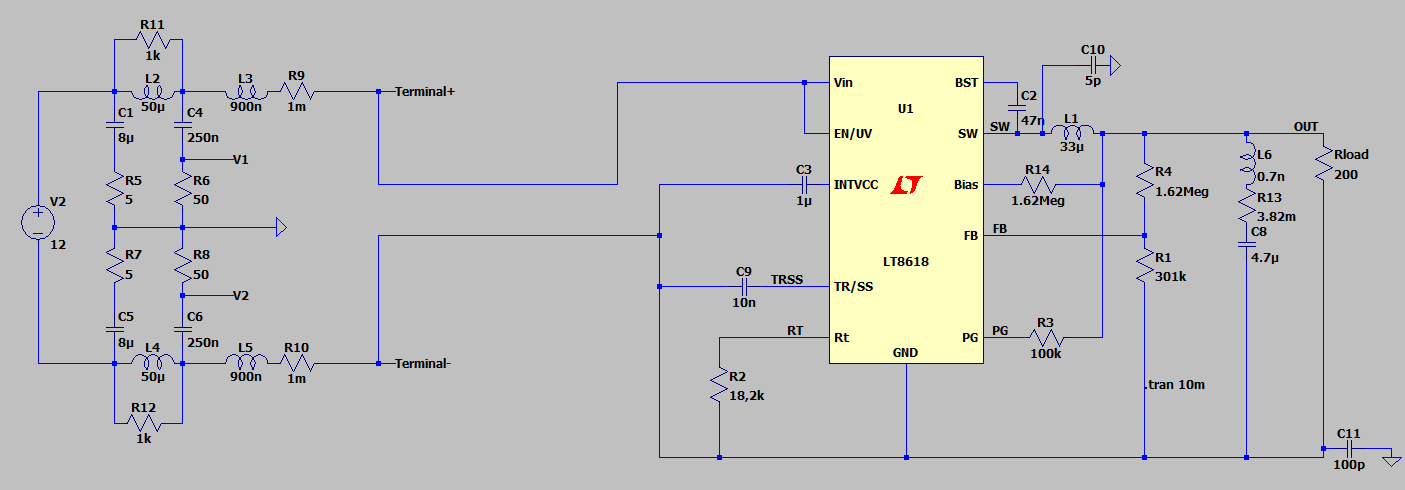
\includegraphics[width=0.8\textwidth]{img/schematic_no_nothing.png}
    \caption{Schematic: \GLS{acr:lisn} and buck converter in their basic setup}
    \label{fig:no_nothing_schematic}
\end{figure}

\begin{figure}[h]
    \centering
    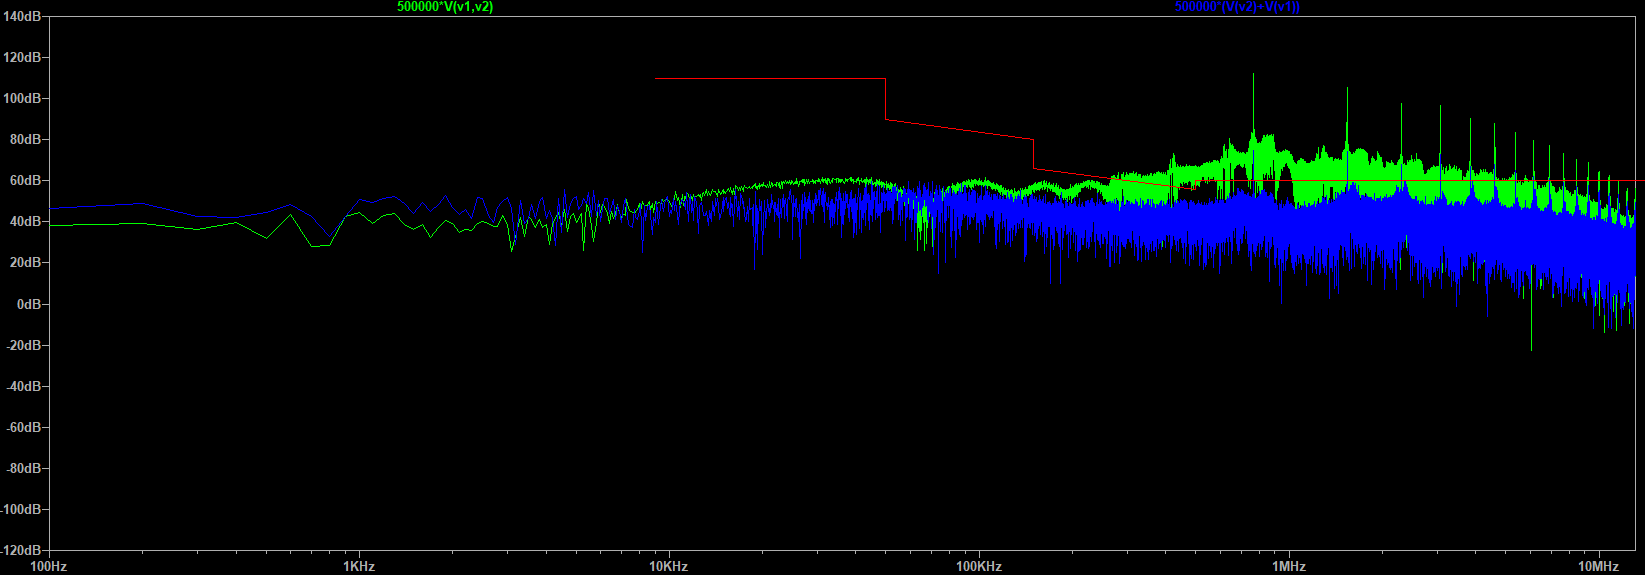
\includegraphics[width=0.8\textwidth]{img/emc_no_nothing.png}
    \caption{conducted emissions of the buck converter - \GLS{acr:dm} in green and \GLS{acr:cm} in blue, red line represents the conducted emissions limit}
    \label{fig:no_nothing_emc}
\end{figure}



% EOF
	% !TEX TS-program = pdflatex
% !TEX encoding = UTF-8 Unicode
% !TEX root = ../main.tex
% !TEX spellcheck = en-US
% ****************************************************************************************
% File: methods.tex
% Author: Jakob Spindler
% Date: 2024-10-16
% ****************************************************************************************
\chapter{Methods}
\label{chapter:methods}

To lower the conducted emissions of the buck converter, the following steps are taken:
\begin{itemize}
    \item place a capacitor at the buck converters input between rails (also known as x-cap) to reduce the \GLS{acr:dm} emissions \autocite{HowGetBest}
    \item implement a \gls{acr:cmc} to reduce the \GLS{acr:cm} emissions \autocite{HowGetBest}
    \item place capacitors between the rails and ground (also known as y-caps) to reduce the \GLS{acr:cm} emissions \autocite{hegartyHowActiveEMI2023}
\end{itemize}



in practice, many other methods can be used to reduce the conducted emissions of a buck converter, such as the use of ferrite beads/cores or even active filtering to name a few \autocite{hegartyHowActiveEMI2023,damnjanovicComparisonDifferentStructures2006}. However, the above-mentioned methods are chosen for their simplicity and cost-effectiveness.


% EOF
    % !TEX TS-program = pdflatex
% !TEX encoding = UTF-8 Unicode
% !TEX root = ../main.tex
% !TEX spellcheck = en-US
% ****************************************************************************************
% File: results.tex
% Author: Jakob Spindler
% Date: 2024-10-16
% ****************************************************************************************
\chapter{Results}
\label{chapter:results}
The following chapter presents the results of the conducted emissions of the buck converter after the implementation of the afforementioned methods.

\section{Rail to Rail X-Cap}
\label{section:x_cap} 
A \qty{22}{\micro\farad} low ESL low ESR Capacitor (C7) is placed between the rails of the buck converter \autocite{885012209006WurthElektronik}.

\begin{figure}[htbp]
    \centering
    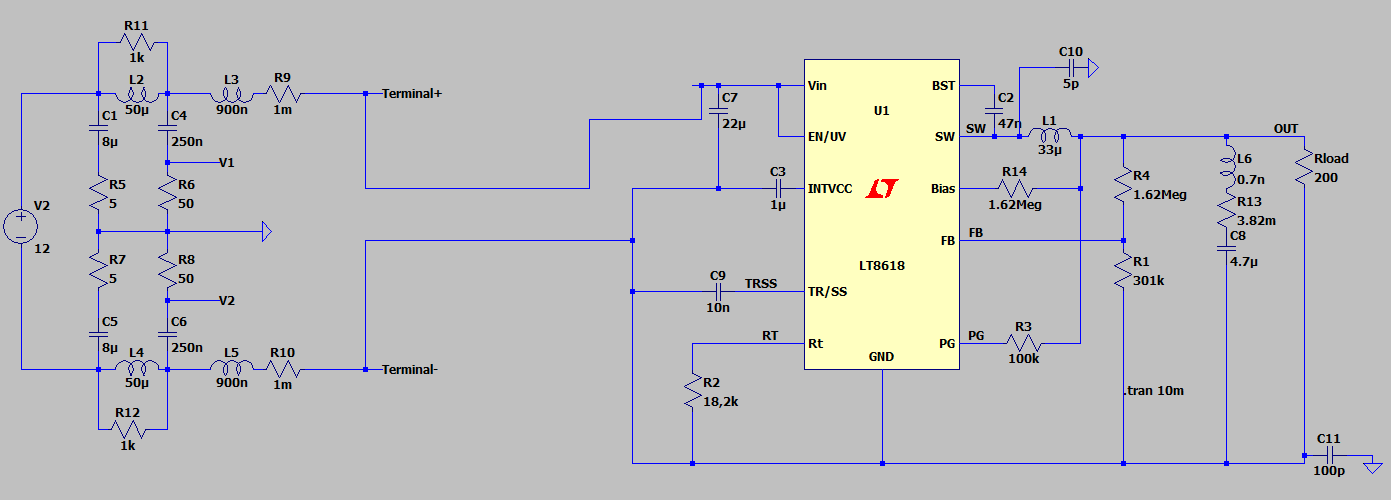
\includegraphics[width=0.8\textwidth]{img/schematic_no_cmc_22u_x_cap.png}
    \caption{Schematic: \GLS{acr:lisn} and buck converter with a rail to rail x-cap}
    \label{fig:x_cap_schematic}
\end{figure}

\begin{figure}[htbp]
    \centering
    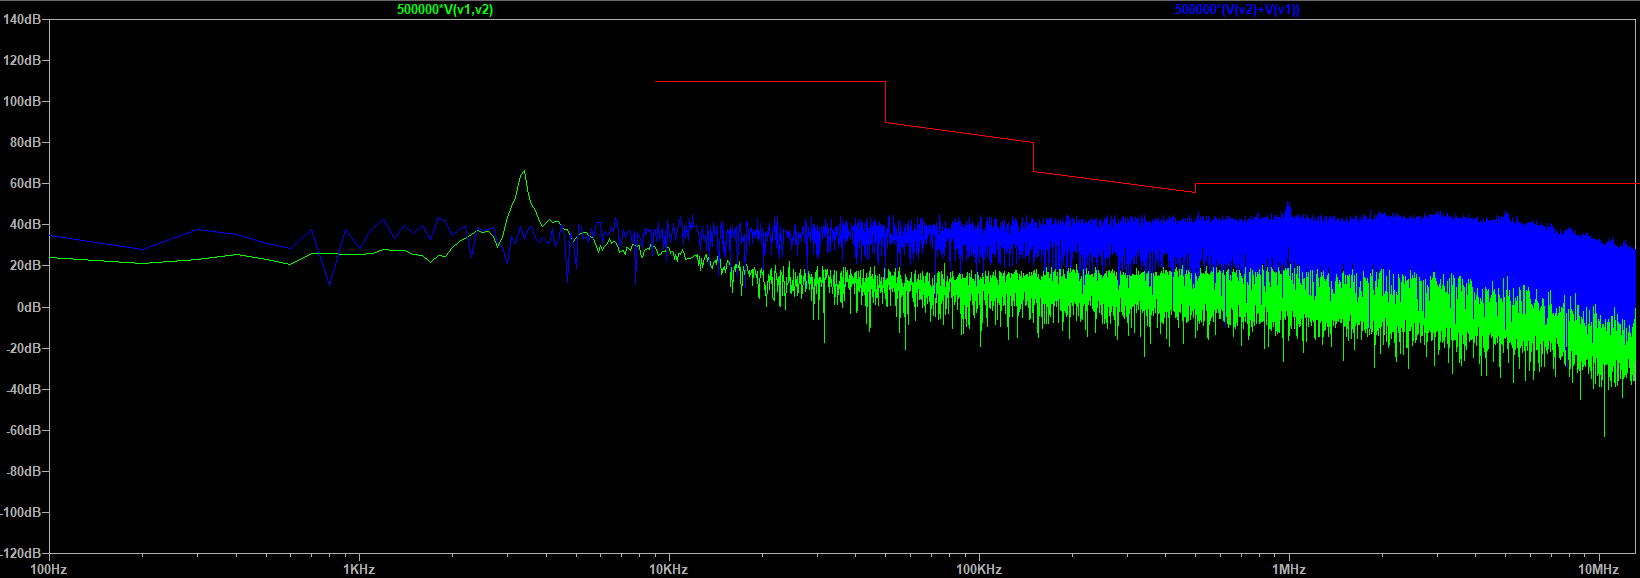
\includegraphics[width=0.8\textwidth]{img/emi_no_cmc_22u_x_cap.png}
    \caption{Conducted emissions of the buck converter with a rail to rail x-cap with \GLS{acr:dm} in green and \GLS{acr:cm} in blue, red line represents the conducted emissions limit}
    \label{fig:x_cap_emc}
\end{figure}

\begin{figure}
    \centering
    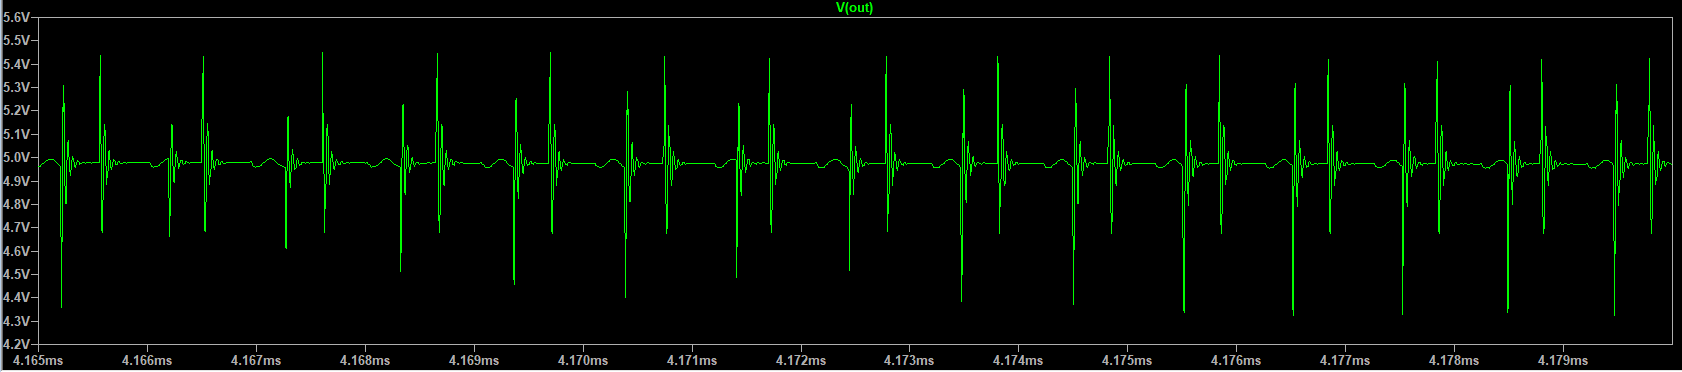
\includegraphics[width=0.8\textwidth]{ripple_22u_x_cap.png}
    \caption{steady state output voltage ripple of the buck converter with a rail to rail x-cap}
    \label{fig:x_cap_ripple}
\end{figure}

\section{Common Mode Choke and X-Cap}
\label{section:cmc_x_cap}
Additionally to the C7 X-Cap a \qty{250}{\micro\henry} common mode choke (L7) is placed on the rails \autocite{744235251WurthElektronik}.

\begin{figure}[htbp]
    \centering
    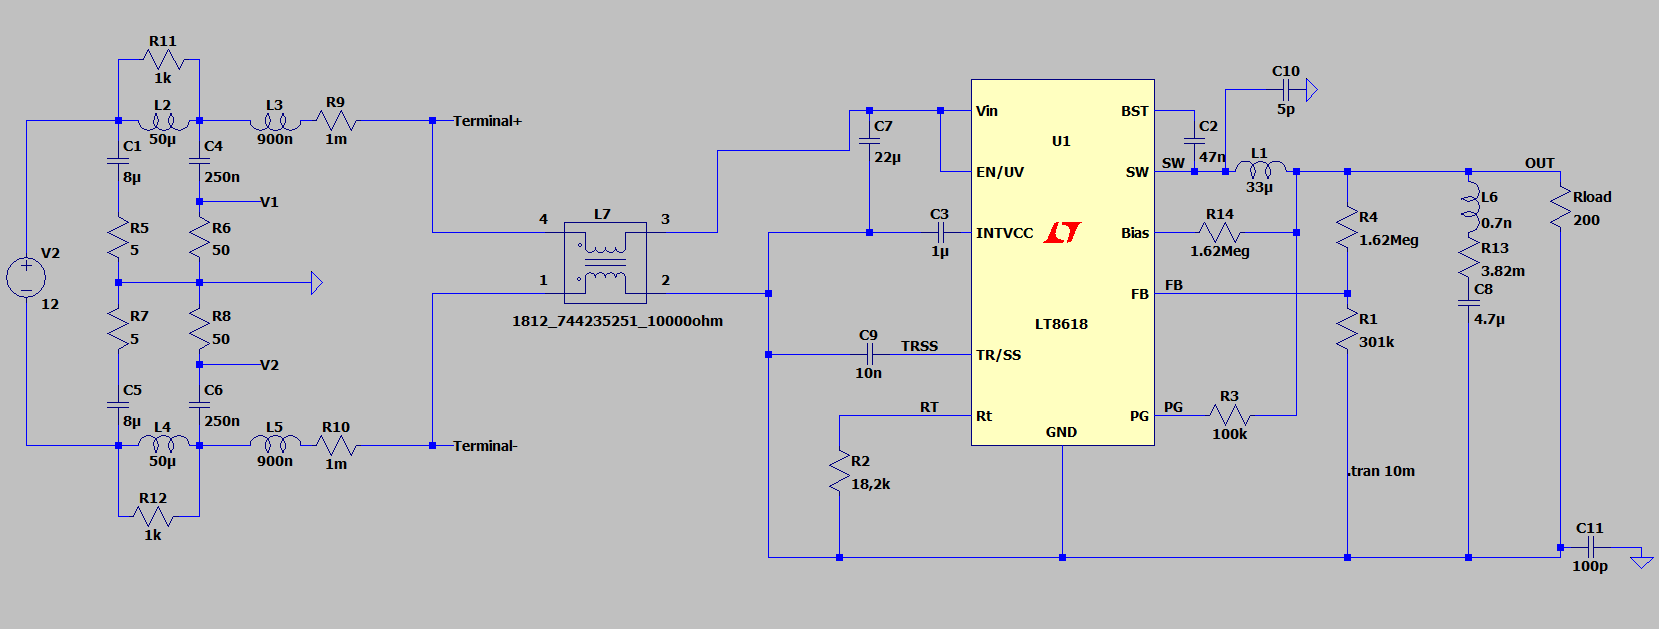
\includegraphics[width=0.8\textwidth]{img/schematic_cmc_22u_x_cap.png}
    \caption{Schematic: \GLS{acr:lisn} and buck converter with a rail to rail x-cap and a common mode choke}
    \label{fig:cmc_x_cap_schematic}
\end{figure}

\begin{figure}[htbp]
    \centering
    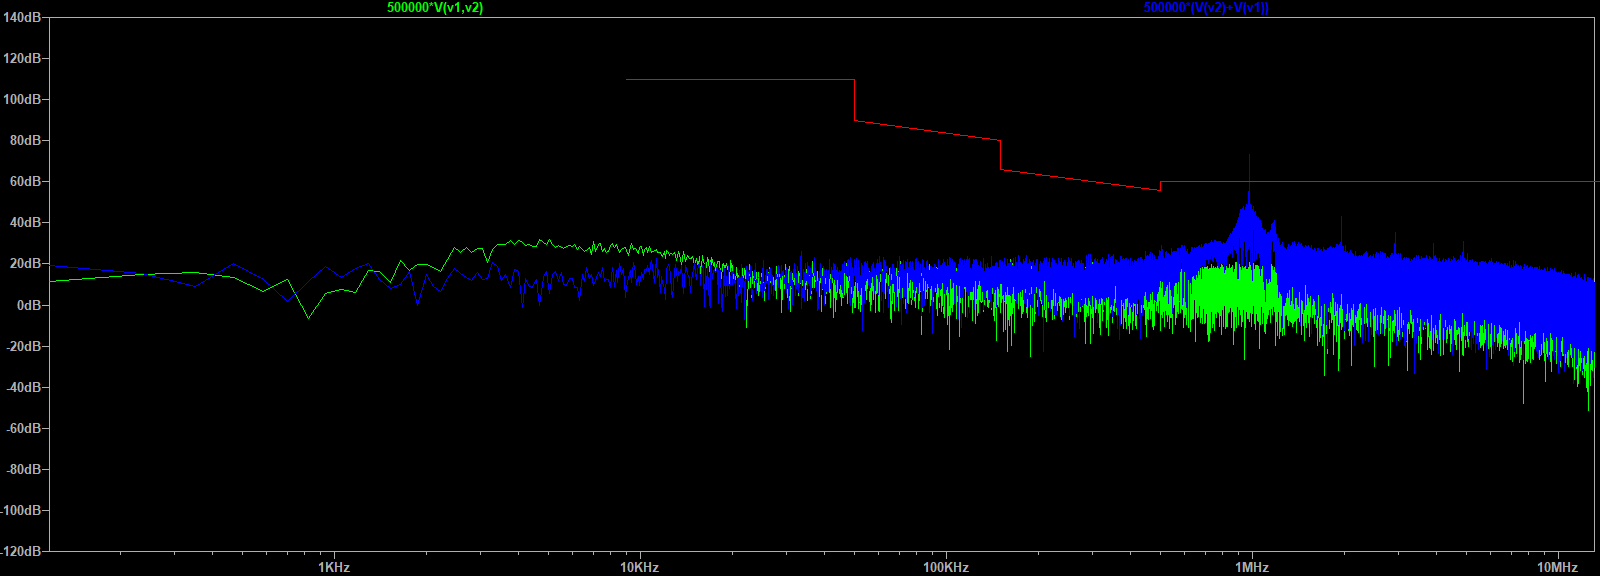
\includegraphics[width=0.8\textwidth]{img/emi_cmc_22u_x_cap.png}
    \caption{Conducted emissions of the buck converter with a rail to rail x-cap and a common mode choke with \GLS{acr:dm} in green and \GLS{acr:cm} in blue, red line represents the conducted emissions limit}
    \label{fig:cmc_x_cap_emc}
\end{figure}

\newpage

\section{Common Mode Choke, X-Cap and Y-Caps}
\label{section:cmc_x_cap_y_cap}

In addition to the C7 X-Cap and the L7 Common Mode Choke, \qty{10}{\nano\farad} Y-Caps (C12, C13) are placed between the rails and ground.

\begin{figure}[htbp]
    \centering
    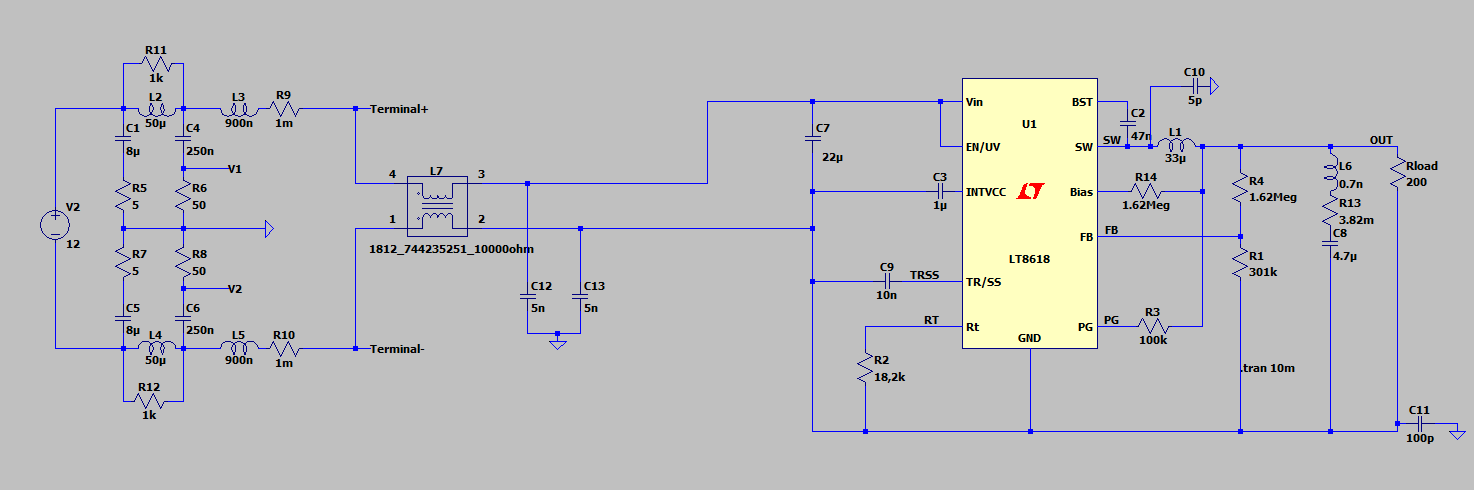
\includegraphics[width=0.8\textwidth]{img/schematic_cmc_x_cap_and_y_caps.png}
    \caption{Schematic: \GLS{acr:lisn} and buck converter with a rail to rail x-cap, a common mode choke and y-caps}
    \label{fig:cmc_x_cap_y_cap_schematic}
\end{figure}

\begin{figure}[htbp]
    \centering
    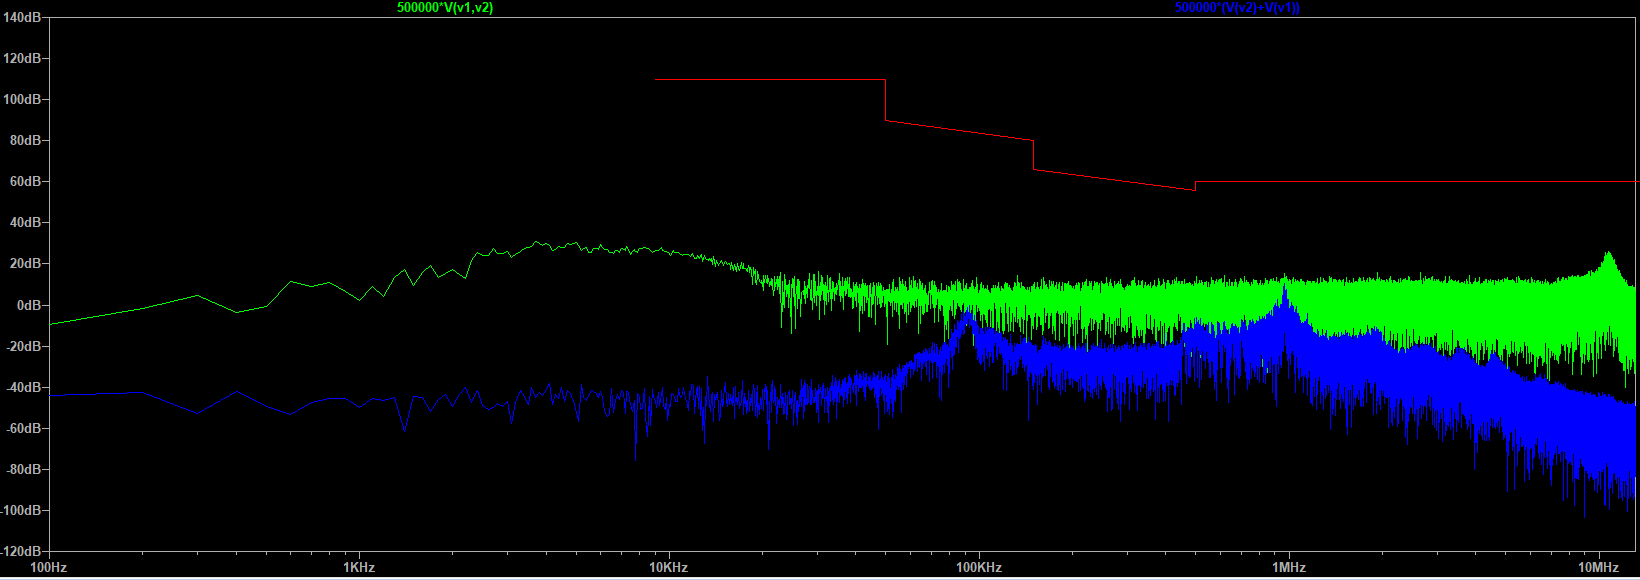
\includegraphics[width=0.8\textwidth]{img/emc_cmc_x_cap_and_y_caps.png}
    \caption{Conducted emissions of the buck converter with a rail to rail x-cap, a common mode choke and y-caps with \GLS{acr:dm} in green and \GLS{acr:cm} in blue, red line represents the conducted emissions limit}
    \label{fig:cmc_x_cap_y_cap_emc}
\end{figure}

\begin{figure}[htbp]
    \centering
    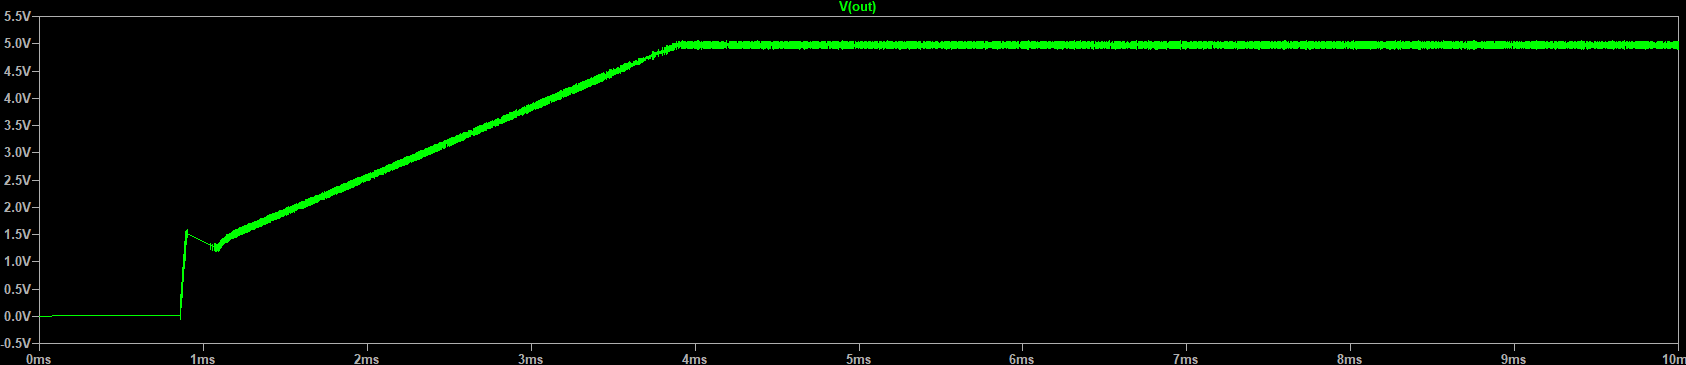
\includegraphics[width=0.8\textwidth]{img/vout_cmc_x_cap_and_y_caps.png}
    \caption{Output voltage of the buck converter with a rail to rail x-cap, a common mode choke and y-caps}
    \label{fig:cmc_x_cap_y_cap_vout}
\end{figure}




% EOF
    % !TEX TS-program = pdflatex
% !TEX encoding = UTF-8 Unicode
% !TEX root = ../main.tex
% !TEX spellcheck = en-US
% ****************************************************************************************
% File: discussion.tex
% Author: Jakob Spindler
% Date: 2024-10-16
% ****************************************************************************************
\chapter{Discussion}
\label{chapter:discussion}

The Results show that the use of an X-cap alone is sufficient enough to reduce the conducted emissions of the buck converter to a level that is compliant with the EN 55022/32 standard. This implementation is also the most cost-effective and simplest to implement, however, it creates a high output voltage ripple/spiking that spans aproxiamtely \qty{1}{\volt} as can be seen in \autoref{fig:x_cap_ripple}. This ripple is not ideal for sensitive applications and may require further filtering.

The use of a \gls{acr:cmc} in addition to the X-cap further reduces the overall emissions, but the difference is marginal. Additionally, a substantial spike in \gls{acr:cm} emissions is observed at \qty{1}{\mega\hertz} as can be seen in \autoref{fig:cmc_x_cap_emc}. This spike is likely due to the resonance of the \gls{acr:cmc} and the parasitic capacitance of the buck converter and leads to a no-pass criterion for the EN 55022/32 standard.

The use of Y-caps in addition to the X-cap and the \gls{acr:cmc} reduces the conducted \gls{acr:cm} emissions of the buck converter which are now well below the limit of the EN 55022/32 standard. The output voltage ripple is also reduced to a level that is acceptable for sensitive applications as can be seen in \autoref{fig:cmc_x_cap_y_cap_vout}.

In conclusion, the use of an X-cap alone is sufficient to reduce the conducted emissions of the buck converter to an acceptable level. 
By implementing a \gls{acr:cmc} and Y-caps in addition to the X-cap, the emissions can be further reduced whilst also reducing the output voltage ripple.

\section{PCB Layout Considerations}
\label{section:pcb_layout_considerations}
For our implemented methods to be efficte in a real world scenario, a fitting \Gls{acr:pcb} layout is crucial. The following points should be considered\autocite{LT8618DatasheetProduct}:
\begin{itemize}
    \item Place the input capacitor (CIN) adjacent to the VIN and GND pins to minimize the loop formed by the input capacitor.
    \item If using a large input capacitor, place a small case/value capacitor close to the VIN and GND pins and the larger capacitor further away.
    \item Place the inductor and output capacitor (COUT) on the same side of the circuit board as the input capacitor.
    \item Ensure connections for the input capacitor, inductor, and output capacitor are made on the same layer.
    \item Place a local, unbroken ground plane under the application circuit on the layer closest to the surface layer.
    \item Keep the SW and BOOST nodes as small as possible.
    \item Keep the FB and RT nodes small and shield them from the SW and BOOST nodes with ground traces.
    \item Route the SYNC node below the ground plane to minimize capacitive coupling to the FB and TR/SS nodes.
    \item Solder the exposed pad on the bottom of the package to ground for electrical connection and thermal heat sinking.
    \item Extend the ground plane as much as possible and add thermal vias near the LT8618 family to additional ground planes within the circuit board and on the bottom side.
\end{itemize}



\begin{figure}[htbp]
    \centering
    \begin{subfigure}[b]{0.45\textwidth}
        \centering
        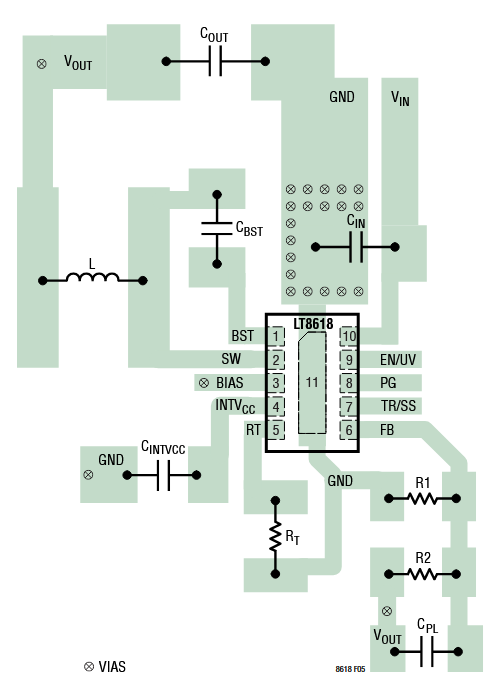
\includegraphics[width=\textwidth]{pcb_layout_LT8618.png}
        %\caption{recommended \gls{acr:pcb} layout of the LT8618 buck converter \autocite{LT8618DatasheetProduct}}
        \label{fig:pcb_layout_LT8618}
    \end{subfigure}
    \hfill
    \begin{subfigure}[b]{0.45\textwidth}
        \centering
        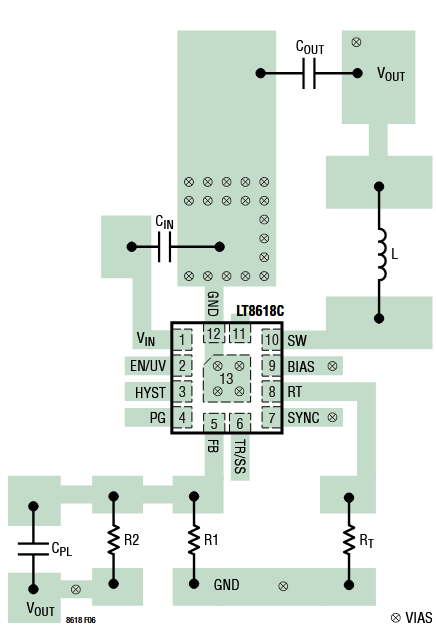
\includegraphics[width=\textwidth]{pcb_layout_LT8618C.png}
        %\caption{recommended \gls{acr:pcb} layout of the LT8618C buck converter \autocite{LT8618DatasheetProduct}}
        \label{fig:pcb_layout_LT8618C}
    \end{subfigure}
    \caption{Recommended PCB layouts for the LT8618 (a) and LT8618C (b) buck converter \autocite{LT8618DatasheetProduct}}
\end{figure}

% \begin{figure}
%     \centering
%     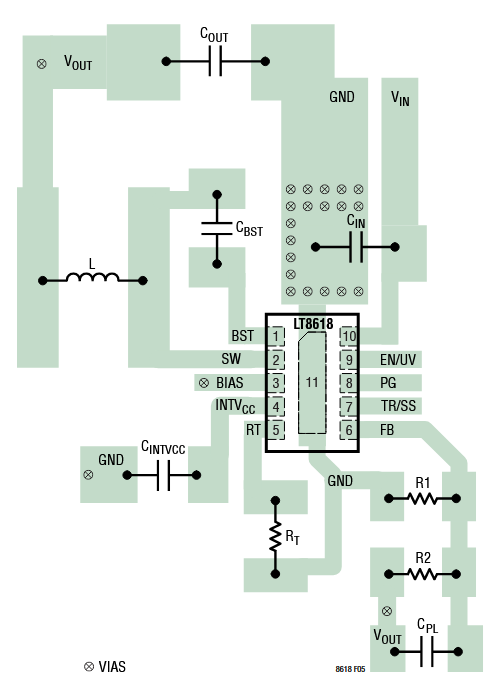
\includegraphics[width=0.8\textwidth]{pcb_layout_LT8618.png}
%     \caption{recommended \gls{acr:pcb} layout of the LT8618 buck converter \autocite{LT8618DatasheetProduct}}
%     \label{fig:pcb_layout_LT8618}
% \end{figure}

% \begin{figure}
%     \centering
%     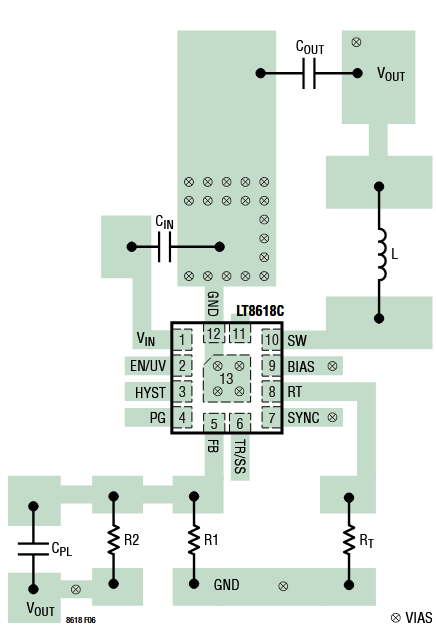
\includegraphics[width=0.8\textwidth]{pcb_layout_LT8618C.png}
%     \caption{recommended \gls{acr:pcb} layout of the LT8618C buck converter \autocite{LT8618DatasheetProduct}}
%     \label{fig:pcb_layout_LT8618C}
% \end{figure}


% EOF

	\pagenumbering{Roman}
	\setcounter{page}{\value{romanpagecount}}
	\stepcounter{page}
	%\bibliography{bib}
	\printbibliography[heading=bibintoc] % This will add the bibliography to the table of contents
    
	%\addcontentsline{toc}{chapter}{\bibname}
	\listoffigures
	\addcontentsline{toc}{chapter}{\listfigurename}
	%\listoftables
	%\addcontentsline{toc}{chapter}{\listtablename}
	
 
	\clearpage
	\printglossary[type=\acronymtype] % input files created by makeindex
	\printglossary[type=symbolslist,style=symbolsliststyle] % input files created by makeindex

	\appendix
	% !TEX TS-program = pdflatex
% !TEX encoding = UTF-8 Unicode
% !TEX root = ../main.tex
% !TEX spellcheck = en-US
% ****************************************************************************************
% File: appendix.tex
% Author: Jakob Spindler
% Date: 2024-10-16
% ****************************************************************************************
\chapter{Appendix}
\label{chapter:Appendix}

\section{Plot file for LTSpice}

\begin{lstlisting}[language=TeX]
[FFT of time domain data]
{
    Npanes: 1
    {
        traces: 2 {2,0,"500000*V(v1,v2)"} {3,0,"500000*(V(v2)+V(v1))"}
        X: ('M',0,10000,0,3e+007)
        Y[0]: (' ',0,1,20,1e+006)
        Y[1]: (' ',0,1,20,1e+006)
        Log: 1 2 0
        PltMag: 1
        Line: "dB" 4 0 (9000,316227.766016838) (50000,316227.766016838)
        Line: "dB" 4 0 (50000,316227.766016838) (50000,31622.7766016838)
        Line: "dB" 4 0 (50000,31622.7766016838) (150000,10000)
        Line: "dB" 4 0 (150000,10000) (150000,1995.26231496888)
        Line: "dB" 4 0 (150000,1995.26231496888) (500000,630.957344480193)
        Line: "dB" 4 0 (500000,630.957344480193) (500000,630.957344480193)
        Line: "dB" 4 0 (500000,630.957344480193) (500000,1000)
        Line: "dB" 4 0 (500000,1000) (30000000,1000)
    }
}
\end{lstlisting}




\end{document}
% EOF